\section{Use-Case-Modell}
\subsection{Use-Case-Diagramm}
\begin{figure}[H]
    \centering
    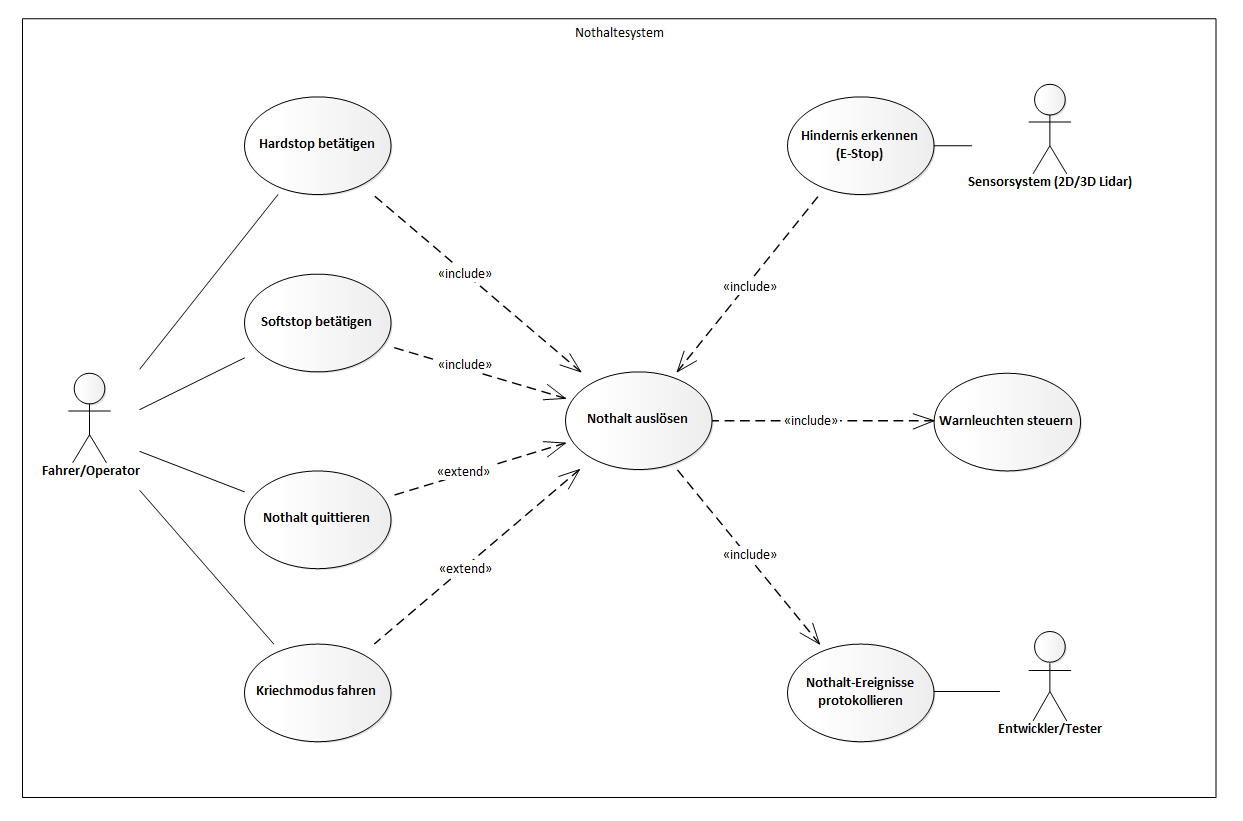
\includegraphics[width=0.9\textwidth]{images/Nothalt_USECASE_Diagramm.png}
    \caption{Use-Case-Diagramm des Nothaltesystems}
    \label{fig:use_case_diagram}
\end{figure}

\subsection{Beschreibung}
Das Use-Case-Diagramm zeigt alle relevanten Interaktionen, beteiligten Akteure
sowie die funktionalen Abläufe, die im Rahmen des Nothaltesystems eines
autonomen Nutzfahrzeugs unterstützt werden. Ziel des Modells ist es, die
externen Sichtweisen auf das System klar zu strukturieren und die wesentlichen
Funktionen – insbesondere das Auslösen und Verarbeiten eines Nothalts –
übersichtlich darzustellen.

\subsection{Akteure}
\textbf{Fahrer / Operator}\\
Der Fahrer bzw. Operator ist der primäre menschliche Nutzer des Systems. Er kann
\ac{Hardstop} und \ac{Softstop} auslösen, den Nothalt quittieren sowie den Kriechmodus für
kontrollierte Bewegungen nach einem Nothalt anfordern.

\textbf{Sensorsystem (2D/3D LiDAR)}\\
Das Sensorsystem repräsentiert die automatisierte Hinderniserkennung. Es agiert
als externer Auslöser eines Nothalts, indem es kritische Objekte oder Gefahren
erkennt und dadurch die Funktion „Nothalt auslösen“ anstößt.

\textbf{Entwickler / Tester}\\
Dieser Akteur steht für Personal, das das System überwacht, Tests durchführt und
Zugang zu den protokollierten Nothalt-Ereignissen benötigt.


\subsection{Beschreibung der Use Cases}

\textbf{\ac{Hardstop} betätigen}\\
Der \ac{Hardstop} wird durch Betätigung eines Not-Aus-Tasters aktiviert. Diese Aktion
führt zwingend zur Aktivität „Nothalt auslösen“. Der \ac{Hardstop} ist ein
sicherheitskritisches, sofort wirkendes Ereignis.\\
\textit{Beziehung: include → Nothalt auslösen}

\vspace{0.5em}

\textbf{\ac{Softstop} betätigen}\\
Der \ac{Softstop} wird über ein Bedienelement ausgelöst und führt ebenfalls zu einem
Nothalt, jedoch ohne sofortiges Trennen der Energieversorgung.\\
\textit{Beziehung: include → Nothalt auslösen}

\vspace{0.5em}

\textbf{Hindernis erkennen (E-Stop)}\\
Das Sensorsystem erkennt ein Hindernis, erzeugt ein E-Stop-Signal und initiiert
unmittelbar die Funktion „Nothalt auslösen“.\\
\textit{Beziehung: include → Nothalt auslösen}

\vspace{0.5em}

\textbf{Nothalt auslösen}\\
Dies ist der zentrale Use Case des Systems. Er umfasst alle
sicherheitsrelevanten Reaktionen wie das sofortige Stoppen des Fahrzeugs, das
Aktivieren der Warnleuchten sowie das Protokollieren relevanter
Ereignisdaten.\\
\textit{Beziehungen:}
\begin{itemize}
    \item include → Warnleuchten steuern
    \item include → Nothalt-Ereignisse protokollieren
\end{itemize}

\vspace{0.5em}

\textbf{Warnleuchten steuern}\\
Dieser Use Case aktiviert oder deaktiviert externe optische Signale, welche den
Nothalt nach außen anzeigen.

\vspace{0.5em}

\textbf{Nothalt-Ereignisse protokollieren}\\
Hierbei werden Zeitpunkt, Auslöser, Systemstatus und weitere
sicherheitsrelevante Informationen aufgezeichnet. Entwickler und Tester nutzen
diese Daten für Diagnose und Validierung.

\vspace{0.5em}

\textbf{Nothalt quittieren}\\
Der Operator bestätigt nach einem Nothalt, dass er die Situation bewertet hat.
Die Quittierung erweitert den zentralen Use Case „Nothalt auslösen“, da sie nur
nach einem ausgelösten Nothalt auftreten kann.\\
\textit{Beziehung: extend ← Nothalt auslösen}

\vspace{0.5em}

\textbf{Kriechmodus fahren}\\
Nach erfolgter Quittierung kann der Operator ein eingeschränktes und
kontrolliertes Fahren im Kriechmodus anfordern. Dieser Use Case erweitert
ausschließlich Situationen nach einem ausgelösten Nothalt.\\
\textit{Beziehung: extend ← Nothalt auslösen}